\documentclass[10pt,letterpaper]{amspset}
\usepackage{fullpage}
\usepackage{gensymb}
\usepackage{graphicx}
\usepackage{tikz}
\usepackage{amsmath}
\usepackage{pgfplots}
\usepackage{amsthm}
\usepackage{amssymb}
\pgfplotsset{compat=1.17}
\graphicspath{ {./images/} }
\notag

% info for header block in upper right hand corner
\name{Brady Lamson}
\class{MATH 1120 SPRING 2021}
\assignment{Inverse Trigonometric Functions Part II}
\duedate{Feb 28th}
\begin{document}

\problemlist{Inverse Trigonometric Functions Part II:  

Section 10.6: 1--4, 13--16, 24--27, 35--38, 41, 42, 45, 46, 49, 50, 53, 54, 57--65, 72--74, 78--80, 131--134, 155--157, 165--168, 181--185, 211--214}

In exercises 1--40, find the exact value.

\begin{problem}[1]
    $\arcsin(-1)$
\end{problem}

\begin{solution}
    Since arcsine is the inverse of sine we can rewrite it as such:
    \begin{align}
        \arcsin(-1) = \theta \\
        \sin(\theta) = -1
    \end{align}
    
    So we just need to find the value of $\theta$ that would satisfy $\sin(\theta) = -1$. There are two values here assuming we don't go beyond $2\pi$. Those values are $\theta = -\frac{\pi}{2}$ and $\theta = -\frac{3\pi}{2}$. Now, our range is actually restricted more than that. Our value can't go beyond $(\pm\ \frac{\pi}{2})$. \footnote{Figure 1 in the reference section explains arcsine more} This means:
    
    \[\boxed{ \arcsin(-1) = -\frac{\pi}{2}  }\]
\end{solution}


\begin{problem}[2]
    $\arcsin(-\frac{ \sqrt{3} } {2})$
\end{problem}

\begin{solution}
    \begin{align}
        \arcsin(-\frac{ \sqrt{3} } {2}) = \theta \\
        \sin(\theta) = -\frac{ \sqrt{3} } {2}
    \end{align}
    
    The above is true is true in one case when the restricted range is taken into account. That one value is $ \theta = -\frac{\pi}{3}$.
    
    \[\boxed{ \theta = -\frac{\pi}{3} }\]
\end{solution}


\pagebreak


\begin{problem}[3]
    $\arcsin(-\frac{ \sqrt{2} } {2})$
\end{problem}

\begin{solution}
    \begin{align}
        \arcsin(-\frac{ \sqrt{2} } {2}) = \theta \\
        \sin(\theta) = -\frac{ \sqrt{2} } {2}
    \end{align}
    
    The above is true is true in one case when the restricted range is taken into account. That one value is $ \theta = -\frac{\pi}{4}$.
    
    \[\boxed{ \theta = -\frac{\pi}{4} }\]
\end{solution}


\begin{problem}[4]
    $\arcsin(-\frac{1}{2})$
\end{problem}

\begin{solution}
    \begin{align}
        \arcsin(-\frac{1}{2}) = \theta \\
        \sin(\theta) = -\frac{1}{2}
    \end{align}
    
    The above is true is true in one case when the restricted range is taken into account. That one value is $ \theta = -\frac{\pi}{6}$.
    
    \[\boxed{ \theta = -\frac{\pi}{6} }\]
\end{solution}

\begin{problem}[13]
    $\arccos(-\frac{1}{2})$
\end{problem}

\begin{solution}
    Alright as always do not overcomplicate this! In reality this is simply asking what values of $\theta$ would satisfy $cos(\theta) = -\frac{1}{2}$. We can, and should, utilize the unit circle for these problems. Considering our restricted range\footnote{Figure 1} of $\pm 1$ only one value satisfies what we need, and that is $\frac{2\pi}{3}$.
    
    \[\boxed{ \theta = -\frac{2\pi}{3} }\]
\end{solution}


\begin{problem}[14]
    $\arccos(0)$
\end{problem}

\begin{solution}
    \[ \arccos(0) = \theta \]
    \[ \cos(\theta) = 0\]
    \[ \theta = \frac{\pi}{2} or \frac{3\pi}{2}\]
    \[ \boxed{ \theta = \frac{\pi}{2} }\]
\end{solution}


\pagebreak


\begin{problem}[15]
    $\arccos(\frac{1}{2})$
\end{problem}

\begin{solution}
    \[ \arccos(\frac{1}{2}) = \theta \]
    \[ \cos(\theta) = \frac{1}{2}\]
    \[ \theta = \frac{\pi}{3} or \frac{5\pi}{3}\]
    \[ \boxed{ \theta = \frac{\pi}{3} }\]
\end{solution}


\begin{problem}[16]
    $\arccos(\frac{\sqrt{2}}{2})$
\end{problem}

\begin{solution}
    \[ \arccos(\frac{\sqrt{2}}{2}) = \theta \]
    \[ \cos(\theta) = \frac{\sqrt{2}}{2}\]
    \[ \theta = \frac{\pi}{4} or \frac{7\pi}{3}\]
    \[ \boxed{ \theta = \frac{\pi}{4} }\]
\end{solution}


\begin{problem}[24]
    $\arctan(1)$
\end{problem}

\begin{solution}
    This is the same process but with one extra step. Just remember that $tan(\theta) = \frac{\sin(\theta)}{\cos(\theta)}$ 
    \[ \arctan(1) = \theta \]
    \[ \tan(\theta) = 1\]
    
    When tangent of $\theta$ is 1 we know based on tangents definition that both sine and cosine need to be the same to get 1. This gives us one result given our restrictions\footnote{Figure 2} of $\pm \frac{\pi}{2}$. 
    
    \[ \boxed{ \theta = \frac{\pi}{4} }\]
\end{solution}


\pagebreak


\begin{problem}[25]
    $\arctan(\sqrt{3})$
\end{problem}

\begin{solution}
    \[ \arctan(\sqrt{3}) = \theta \]
    \[ \tan(\theta) = \sqrt{3}\]
    \[ \frac{\sin(\theta)}{\cos(\theta)} = \sqrt{3} \]
    
    Okay, so looking at the unit circle we can see one easy answer here. $\frac{\pi}{3}$ has a sine and a cosine that equal just that! $sin(\frac{\pi}{3}) = \frac{\sqrt{3}}{2}$ and $cos(\frac{\pi}{3}) = \frac{1}{2}$.
    
    \[ \frac{ \frac{\sqrt{3}}{2} } { \frac{1}{2} } = \sqrt{3} \]
    \[\boxed{ \theta = \frac{\pi}{3} } \]
\end{solution}


\begin{problem}[26]
    $arccot(-\sqrt{3})$
\end{problem}

\begin{solution}
    This is basically the same as the previous problem, it's just working with cotangent and a negative value instead! Remember, cotangent is $\frac{cos(\theta}{sin(\theta)}$ which is tangent but flipped. 
    
    From here we just need to do what we did for the previous problem, but keeping in consideration the different range restriction of cotangent which is $0 \rightarrow 1\pi$. Just looking at the unit circle it quickly becomes clear what we need is $\theta = \frac{\pi}{6}$.
    
    \[ cot(\frac{\pi}{6}) =  \frac{ -\frac{\sqrt{3}}{2} } { \frac{1}{2} } = -\sqrt{3}\]
    \[\boxed{ arccot(-\sqrt{3}) = \frac{\pi}{6} }\]
\end{solution}


\begin{problem}[27]
    $arccot(-1)$
\end{problem}

\begin{solution}
    Same general process as problem 24 will be applied here. $\frac{3\pi}{4}$ will be our answer here. Dividing cosine by sine in this instance results in -1.  
    
    \[ \frac{ -\frac{ \sqrt{2} }{2} } { \frac{ \sqrt{2} }{2} } = -1\]
    \[ arccot(-1) = \frac{3\pi}{4}\]
\end{solution}


\pagebreak


\begin{problem}[35]
    $arcsec(\sqrt{2})$
\end{problem}

\begin{solution}
    So, secant is $\frac{1}{cosine}$. From here we can pick out a likely candidate. Just looking at the unit circle I think $\frac{\pi}{4}$ is the choice. Let's verify that. We know that $sin(\frac{\pi}{4}) = \frac{ \sqrt{2} } {2}$. Therefore we can do the following calculation. 
    
    \[ \frac{1}{ \frac{\sqrt{2}}{2}  } \] 
    
    We can multiply this by its conjugate ($2\sqrt{2}$) to simplify this. 
    
    \[ \frac{2\sqrt{2}} {\frac{2 \cdot 2}{2}} = \frac{2\sqrt{2}}{2} = \sqrt{2} \]
    
    So, now we know that this is the correct answer! 
    
    \[\boxed{ arcsec(\sqrt{2}) = \frac{\pi}{4} }\]
\end{solution}


\begin{problem}[36]
    $arccsc(\sqrt{2})$
\end{problem}

\begin{solution}
    For this problem we'll be using the exact same methodology. For any questions please refer to the logic used in problem 35. The only difference here is the trig function utilized. We'll be using sine instead of cosine in the denominator! 
    
    Actually, funnily enough no calculations even need to be done. We did all the math in problem 35! Since sine and cosine are the same for $\frac{\pi}{4}$ the exact same logic applies. So I can safely say the following! 
    
     \[\boxed{ arccsc(\sqrt{2}) = \frac{\pi}{4} }\]
\end{solution}


\begin{problem}[37]
    $arcsec \left( \frac{2\sqrt{3}}{3} \right)$
\end{problem}

\begin{solution}
    Following previous logic I will spare you the details. Considering the definition of secant I believe the answer we're looking for is $\frac{\pi}{6}$. Let's do some verification! 
    
    \[ \frac{1}{ \frac{\sqrt{3}}{2}  } \] 
    
    We can multiply this by its conjugate ($2\sqrt{3}$) to simplify this. 
    
    \[ \left( \frac{2\sqrt{3}} {\frac{2 \cdot 3}{2}} \right) = \frac{2\sqrt{3}}{3} \]
    
    \[\boxed{ arcsec \left( \frac{2\sqrt{3}}{3} \right)= \frac{\pi}{6} }\]
\end{solution}


\pagebreak


\begin{problem}[38]
    $arccsc \left( \frac{2\sqrt{3}}{3} \right)$
\end{problem}

\begin{solution}
    Here we do the exact same thing with one slight variation: We just need to use $\frac{\pi}{3}$ instead. Following the calculations and logic from problem 37 we know that this is the answer.
    
    \[\boxed{ arccsc \left( \frac{2\sqrt{3}}{3} \right)= \frac{\pi}{6} }\]
\end{solution}

\hrule \medskip

In exercises 41--42 and 45--46, assume that the range of arcsecant is $\left[ 0 , \frac{\pi}{2} \right) \cup \left[ \pi , \frac{3\pi}{2} \right)$ and that the range of arccosecant is $\left( 0 , \frac{\pi}{2} \right] \cup \left( \pi , \frac{3\pi}{2} \right]$.

\medskip

Essentially, what this means is we will be working within quadrant 1 and quadrant 3. We just need to be careful about what's included and what isn't.
\medskip

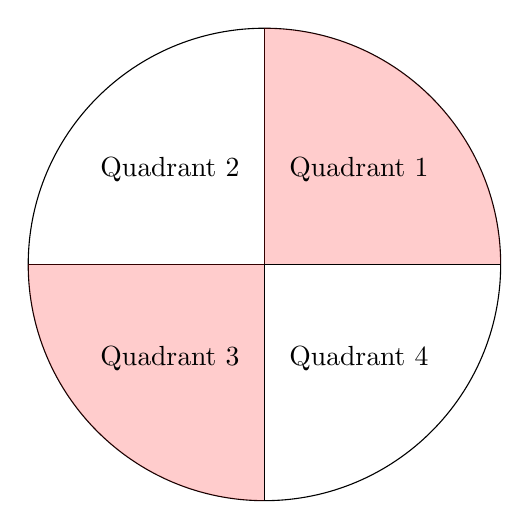
\begin{tikzpicture}
    \draw[clip] (0,0) circle (3);
    \draw (-3,0) -- (3,0);
    \draw (0,3) -- (0,-3);
    \fill[red, fill opacity=0.20] (45:6) rectangle (0,0);
    \fill[red, fill opacity=0.20] (225:6) rectangle (0,0);
    \node[] at (1.2, 1.2) {Quadrant 1};
    \node[] at (-1.2, 1.2) {Quadrant 2};
    \node[] at (-1.2, -1.2) {Quadrant 3};
    \node[] at (1.2, -1.2) {Quadrant 4};
\end{tikzpicture}

\medskip
\hrule


\begin{problem}[41]
    $arcsec(-2)$
\end{problem}

\begin{solution}
    This one isn't too bad. We just need a value of cosine that you can divide 1 by to get -2. That's pretty straight forward, we need a value of $-\frac{1}{2}$. Cosine is only negative in quadrants 2 or 3, and since quadrant 2 is off limits here we have only one choice. 
    
    \[\boxed{  arcsec(-2) = \frac{4\pi}{3}  }\]
\end{solution}


\begin{problem}[42]
    $arcsec(-\sqrt{2})$
\end{problem}

\begin{solution}
    This is a similar situation. We know that $\frac{1}{ \frac{\sqrt{2}}{2} } = \sqrt{2}$. Since the value is negative that means we're restricted to quadrant 3 again. That gives us our answer. 
    
    \[\boxed{ arcsec(-\sqrt{2}) = \frac{5\pi}{4}  }\]
\end{solution}


\pagebreak


\begin{problem}[45]
    $arccsc(-2)$
\end{problem}

\begin{solution}
    This is the exact same dance as problem 41. Only difference here is that we're working with sine, not cosine. So we need a negative sine value of $-\frac{1}{2}$. We're still locked to quadrant 3. As always, that narrows it down enough to say the following.
    
    \[\boxed{ arccsc(-2) = \frac{7\pi}{6}  }\]
\end{solution}


\begin{problem}[46]
    $arccsc(-\sqrt{2})$
\end{problem}

\begin{solution}
    Okay, you know the drill at this point. If you have any questions about my answer please refer to the logic I used in problem 45. We need quadrant 3 and a sine value of $\frac{\sqrt{2}}{2}$. 
    
    \[\boxed{ arccsc(-\sqrt{2}) = \frac{5\pi}{4}   }\]
\end{solution}

\pagebreak
\hrule \medskip

In exercises 49--50 and 53--54, assume that the range of arcsecant is $\left[ 0 , \frac{\pi}{2} \right) \cup \left( \frac{\pi}{2}, \pi \right]$ and that the range of arccosecant is $\left[ 0 , \frac{\pi}{2} \right) \cup \left( \frac{\pi}{2}, \pi \right]$.
\medskip

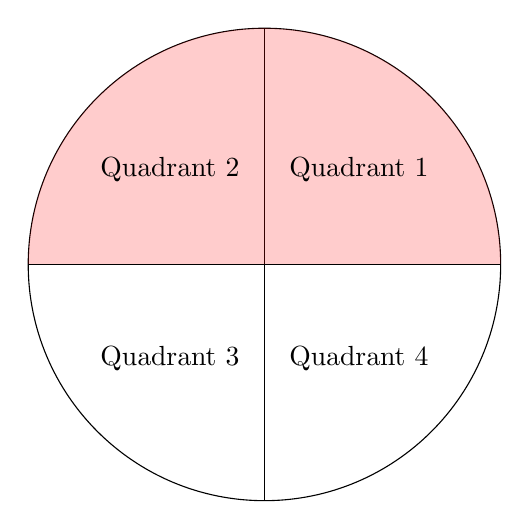
\begin{tikzpicture}
    \draw[clip] (0,0) circle (3);
    \draw (-3,0) -- (3,0);
    \draw (0,3) -- (0,-3);
    \fill[red, fill opacity=0.20] (45:6) rectangle (0,0);
    \fill[red, fill opacity=0.20] (135:6) rectangle (0,0);
    \node[] at (1.2, 1.2) {Quadrant 1};
    \node[] at (-1.2, 1.2) {Quadrant 2};
    \node[] at (-1.2, -1.2) {Quadrant 3};
    \node[] at (1.2, -1.2) {Quadrant 4};
\end{tikzpicture}

\medskip
\hrule


\begin{problem}[49]
    $arcsec(-2)$
\end{problem}

\begin{solution}
    Same dance as problem 41, just a different restriction. We just need a value of cosine that you can divide 1 by to get -2. That's pretty straight forward, we need a value of $-\frac{1}{2}$. Cosine is only negative in quadrants 2 or 3, and since quadrant 3 is off limits here we have only one choice. 
    
    \[\boxed{  arcsec(-2) = \frac{2\pi}{3}  }\]
\end{solution}


\begin{problem}[50]
    $arcsec(-\sqrt{2})$
\end{problem}

\begin{solution}
    Same as problem 42. We know that $\frac{1}{ \frac{\sqrt{2}}{2} } = \sqrt{2}$. Since the value is negative that means we're restricted to quadrant 2 again. That gives us our answer. 
    
    \[\boxed{ arcsec(-\sqrt{2}) = \frac{3\pi}{4}  }\]
\end{solution}


\begin{problem}[53]
    $arccsc(-2)$
\end{problem}

\begin{solution}
    Remember problem 45? Same thing. So we need a negative sine value of $-\frac{1}{2}$. We're still locked to quadrant 2. As always, that narrows it down enough to say the following.
    
    \[\boxed{ arccsc(-2) = \frac{5\pi}{6}  }\]
\end{solution}


\begin{problem}[54]
    $arccsc(-\sqrt{2})$
\end{problem}

\begin{solution}
    Okay, you know the drill at this point. If you have any questions about my answer please refer to the logic I used in problem 46. We need quadrant 2 and a sine value of $\frac{\sqrt{2}}{2}$. 
    
    \[\boxed{ arccsc(-\sqrt{2}) = \frac{3\pi}{4}   }\]
\end{solution}


\hrule \medskip

In exercises 57--65, 72--74, and 78--80, 131--134, 155--157, find the exact value or state that it is undefined. 

\medskip
\hrule

\begin{problem}[57]
    $sin \left(arcsin \left( \frac{1}{2} \right)\right)$
\end{problem}

\begin{solution}
    These problems are actually a lot more simple than they look! Let's first think about what we're solving for with regards to both sine and arcsine normally.
    
    \[ sin(\theta) = x \]
    \[ arcsin(x) = \theta \]
    
    The relationship here makes solving these trivial. With sine, the output of the function is x but we already know x because it's in the function of arcsine. Arcsine may be taking the place of $\theta$ but we're still solving for x like normal. So, we can say the following:
    
    \[ sin \left(arcsin \left( x \right)\right) = x\]
    \[\boxed{ sin \left(arcsin \left( \frac{1}{2} \right)\right) = \frac{1}{2} }\]
\end{solution}


\begin{problem}[58]
    $sin \left(arcsin \left( -\frac{\sqrt{2}}{2} \right)\right)$
\end{problem}

\begin{solution}
    For detailed logic refer to problem 57. 
    
    \begin{align}
        sin(\theta) &= x \\
        arcsin(x) &= \theta \\
        sin \left(arcsin \left( -\frac{\sqrt{2}}{2} \right)\right) &= x 
    \end{align}
    
    \[\boxed{ sin \left(arcsin \left( -\frac{\sqrt{2}}{2} \right)\right) = -\frac{\sqrt{2}}{2} } \]
\end{solution}


\pagebreak


\begin{problem}[59]
    $sin \left(arcsin \left( \frac{3}{5} \right)\right)$
\end{problem}

\begin{solution}
    For detailed logic refer to problem 57. 
    
    \begin{align}
        sin(\theta) &= x \\
        arcsin(x) &= \theta \\
        sin \left(arcsin \left( \frac{3}{5} \right)\right) &= x 
    \end{align}
    
    \[\boxed{ sin \left(arcsin \left( \frac{3}{5} \right)\right) = \frac{3}{5} } \]
\end{solution}


\begin{problem}[60]
    $sin \left(arcsin \left( -0.42 \right)\right)$
\end{problem}

\begin{solution}
    For detailed logic refer to problem 57. 
    
    \begin{align}
        sin(\theta) &= x \\
        arcsin(x) &= \theta \\
        sin \left(arcsin \left( -0.42 \right)\right) &= x 
    \end{align}
    
    \[\boxed{ sin \left(arcsin \left( -0.42 \right)\right) = -0.42 } \]
\end{solution}


\begin{problem}[61]
    $sin \left(arcsin \left( \frac{5}{4} \right)\right)$
\end{problem}

\begin{solution}
    So this one is slightly trickier. Remember the default range of sine before you jump the gun! It's $[-1, 1]$. That means if we get an x value higher than $1$ it's undefined! 
    
    \begin{align}
        sin(\theta) &= x \\
        arcsin(x) &= \theta \\
        sin \left(arcsin \left( \frac{5}{4} \right)\right) &= x \\
        sin \left(arcsin \left( \frac{5}{4} \right)\right) &= \frac{5}{4}
    \end{align}
    
    \[ \frac{5}{4} > 1 \]
    \[\boxed{UNDEFINED}\]
\end{solution}


\pagebreak


\begin{problem}[62]
    $cos \left(arccos \left( \frac{\sqrt{2}}{2} \right)\right)$
\end{problem}

\begin{solution}
    For detailed logic refer to problem 57. 
    
    \begin{align}
        cos(\theta) &= x \\
        arccos(x) &= \theta \\
        cos \left(arccos \left( \frac{\sqrt{2}}{2} \right)\right) &= x 
    \end{align}
    
    \[\boxed{ cos \left(arccos \left( \frac{\sqrt{2}}{2} \right)\right) = \frac{\sqrt{2}}{2} } \]
\end{solution}


\begin{problem}[63]
    $cos \left(arccos \left( -\frac{1}{2} \right)\right)$
\end{problem}

\begin{solution}
    For detailed logic refer to problem 57. 
    
    \begin{align}
        cos(\theta) &= x \\
        arccos(x) &= \theta \\
        cos \left(arccos \left( -\frac{1}{2} \right)\right) &= x 
    \end{align}
    
    \[\boxed{ cos \left(arccos \left( -\frac{1}{2} \right)\right) = -\frac{1}{2} } \]
\end{solution}


\begin{problem}[64]
    $cos \left(arccos \left( \frac{5}{13} \right)\right)$
\end{problem}

\begin{solution}
    For detailed logic refer to problem 57. 
    
    \begin{align}
        cos(\theta) &= x \\
        arccos(x) &= \theta \\
        cos \left(arccos \left( \frac{5}{13} \right)\right) &= x 
    \end{align}
    
    \[\boxed{ cos \left(arccos \left( \frac{5}{13} \right)\right) = \frac{5}{13} } \]
\end{solution}


\pagebreak


\begin{problem}[65]
    $cos \left(arccos \left( -0.998 \right)\right)$
\end{problem}

\begin{solution}
    For detailed logic refer to problem 57. 
    
    \begin{align}
        cos(\theta) &= x \\
        arccos(x) &= \theta \\
        cos \left(arccos \left( -0.998 \right)\right) &= x 
    \end{align}
    
    \[\boxed{ cos \left(arccos \left( -0.998 \right)\right) = -0.998 } \]
\end{solution}


\begin{problem}[72]
    $cot \left(arccot \left( 1 \right)\right)$
\end{problem}

\begin{solution}
    Before we push ahead we have to adjust the range we're working with. This is actually easier now though because cotangent has a range of all real numbers. 
    
    For detailed logic refer to problem 57. 
    
    \begin{align}
        cot(\theta) &= x \\
        arccot(x) &= \theta \\
        cos \left(arccot \left( 1 \right)\right) &= x 
    \end{align}
    
    \[\boxed{ cot \left(arccot \left( 1 \right)\right) = 1 } \]
\end{solution}


\begin{problem}[73]
    $cot \left(arccot \left( -\sqrt{3} \right)\right)$
\end{problem}

\begin{solution}
    For detailed logic refer to problems 57 and 72. 
    
    \begin{align}
        cot(\theta) &= x \\
        arccot(x) &= \theta \\
        cos \left(arccot \left( -\sqrt{3} \right)\right) &= x 
    \end{align}
    
    \[\boxed{ cot \left(arccot \left( -\sqrt{3} \right)\right) = -\sqrt{3} } \]
\end{solution}


\pagebreak


\begin{problem}[74]
    $cot \left(arccot \left( -\frac{7}{24} \right)\right)$
\end{problem}

\begin{solution}
    For detailed logic refer to problems 57 and 72. 
    
    \begin{align}
        cot(\theta) &= x \\
        arccot(x) &= \theta \\
        cos \left(arccot \left( -\frac{7}{24} \right)\right) &= x 
    \end{align}
    
    \[\boxed{ cot \left(arccot \left( -\frac{7}{24} \right)\right) = -\frac{7}{24} } \]
\end{solution}


\begin{problem}[78]
    $sec \left(arcsec \left( -1 \right)\right)$
\end{problem}

\begin{solution}
    Time to readjust our range again, except this time it will end up mattering. The range of secant is \linebreak $(-\infty, -1] \cup [1, \infty)$.
    
    For detailed logic refer to problem 57. 
    
    \begin{align}
        sec(\theta) &= x \\
        arcsec(x) &= \theta \\
        sec \left(arcsec \left( -1 \right)\right) &= x 
    \end{align}
    
    \[\boxed{ sec \left(arcsec \left( -1 \right)\right) = -1 } \]
\end{solution}


\begin{problem}[79]
    $sec \left(arcsec \left( \frac{1}{2} \right)\right)$
\end{problem}

\begin{solution}
    For detailed logic refer to problems 57 and 78. 
    
    \begin{align}
        sec(\theta) &= x \\
        arcsec(x) &= \theta \\
        sec \left(arcsec \left( \frac{1}{2} \right)\right) &= x 
    \end{align}
    
    $\frac{1}{2}$ does not fit into the range of secant.
    
    \[\boxed{UNDEFINED} \]
\end{solution}


\pagebreak


\begin{problem}[80]
    $sec \left(arcsec \left( 0.75 \right)\right)$
\end{problem}

\begin{solution}
    For detailed logic refer to problems 57 and 78. 
    
    \begin{align}
        sec(\theta) &= x \\
        arcsec(x) &= \theta \\
        sec \left(arcsec \left( 0.75 \right)\right) &= x 
    \end{align}
    
    $0.75$ does not fit into the range of secant.
    
    \[\boxed{UNDEFINED} \]
\end{solution}


\begin{problem}[131]
    $sin \left( arccos \left( -\frac{1}{2} \right) \right)$
\end{problem}

\begin{solution}
    Okay, so now these get interesting. Not only do we have to play around the limited range of sine, $[-1, 1]$, we also have to figure out what $arccos(x)$ actually is while working within its limited range. Because $arccos(x) = \theta$ once we figure that out we can then find the exact value of $sin(\theta)$. It's not as bad as it sounds though! Remember, arccos has a range of $[0, \pi$], so we're restricted to quadrants 1 and 2. 
    
    \medskip
    
    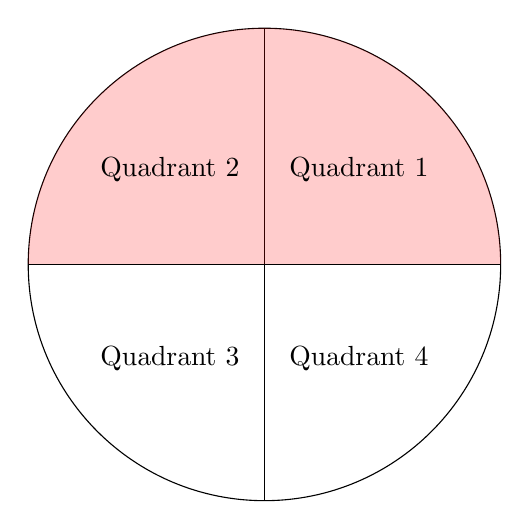
\begin{tikzpicture}
    \draw[clip] (0,0) circle (3);
    \draw (-3,0) -- (3,0);
    \draw (0,3) -- (0,-3);
    \fill[red, fill opacity=0.20] (45:6) rectangle (0,0);
    \fill[red, fill opacity=0.20] (135:6) rectangle (0,0);
    \node[] at (1.2, 1.2) {Quadrant 1};
    \node[] at (-1.2, 1.2) {Quadrant 2};
    \node[] at (-1.2, -1.2) {Quadrant 3};
    \node[] at (1.2, -1.2) {Quadrant 4};
\end{tikzpicture}
    
    \[ arccos\left( -\frac{1}{2} \right) = \frac{2\pi}{3}\]
    \[\boxed{ sin\left( \frac{2\pi}{3} \right) = \frac{\sqrt{3}}{2} }\]
\end{solution}


\pagebreak


\begin{problem}[132]
    $sin \left( arccos \left( \frac{3}{5} \right) \right)$
\end{problem}

\begin{solution}
    Okay, so this problem is working within the same restricted ranges as 131 but that's largely where the similarities end. This is a number that doesn't conveniently fall on the unit circle so we need to go back to basics to be able to solve this. Here's some stuff we know:
    
    \[ arccos\left( \frac{3}{5} \right) = \theta\]
    \[ cos(\theta) = \frac{3}{5} \]
    \[ cos(\theta) = \frac{adjacent}{hypotenuse}\]

    So now we can craft a triangle and go from there! 
    \medskip
    
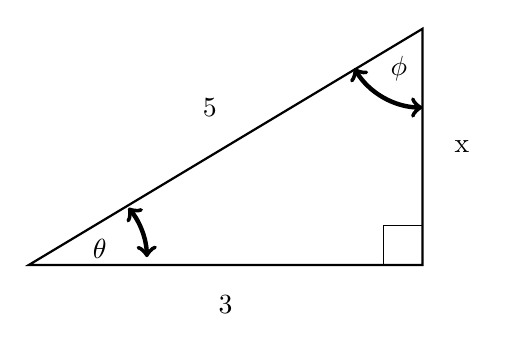
\begin{tikzpicture}
    \draw[black, thick] (0,0) -- (5,0) -- (5,3) -- cycle;
    \draw[ultra thick, <->] (1.5,.1) arc (1:40:1);
    \draw[ultra thick, <->] (5,2) arc (270:210:1);
    % Below nodes are the labels.
        \node[] at (0.9, 0.2) {$\theta$};
        \node[] at (4.7, 2.5) {$\phi$};
        \node[] at (2.5, -0.5) {$3$};
        \node[] at (5.5, 1.5) {x};
        \node[] at (2.3, 2) {5};
    % This draws the right angle.
        \draw(4.5,0)|-(5,.5);
\end{tikzpicture}

Now we solve for x! 

\[ 3^2 + x^2 = 5^2\]
\[ 9 + x^2 = 25 \]
\[ x = \pm 4 \]

One final thing, we know this has to be positive 4. That's because sine is only negative in quadrants 3 and 4 which are off limits.

\[\boxed{ sin(\theta) = \frac{4}{5} }\]
\end{solution}


\pagebreak


\begin{problem}[133]
    $sin(arctan(-2))$
\end{problem}

\begin{solution}
    This is where things get fun. First let's do some work with what we've got. 
    
    \[ arctan(-2) = \theta\]
    \[ tan(\theta) = -2 \]
    
    Okay, so this is the first point where we can figure out stuff. $Tangent(\theta)$ is only negative in two quadrants, 2 and 4. The thing is, cotangent has a range of $(-\frac{\pi}{2}, \frac{\pi}{2})$. This restricts us to quadrants 1 and 4. That means our answer will fall within quadrant 4. In quadrant 4, $cos(\theta)$ is positive and $sin(\theta)$ is negative. This will be important soon. Now let's go a little further! 
    
    \[ tan(\theta) = \frac{sin(\theta)}{cos(\theta)}\]
    \[ -2 = \frac{sin(\theta)}{cos(\theta)}\]
    \[ -2 = \frac{opposite}{adjacent} \]
    
    Now let's make a triangle with that ratio! 
    
    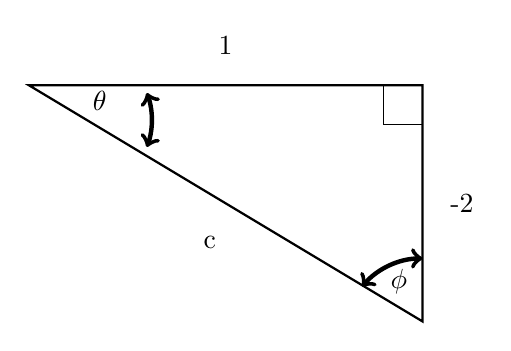
\begin{tikzpicture}
        \draw[black, thick] (0,0) -- (5,0) -- (5,-3) -- cycle;
        \draw[ultra thick, <->] (1.5,-.1) arc (20:-20:1);
        \draw[ultra thick, <->] (5,-2.2) arc (90:140:1);
    % Below nodes are the labels.
        \node[] at (0.9, -0.2) {$\theta$};
        \node[] at (4.7, -2.5) {$\phi$};
        \node[] at (2.5, 0.5) {1};
        \node[] at (5.5, -1.5) {-2};
        \node[] at (2.3, -2) {c};
    % This draws the right angle.
        \draw(4.5,0)|-(5,-.5);
    \end{tikzpicture}

    \[ -2^2 + 1^2 = c^2\]
    \[ 5 = c^2\]
    \[ c = \sqrt{5}\]

    Since sine is $\frac{opposite}{hypotenuse}$ we can say:

    \[ sin(\theta) = -\frac{2}{\sqrt{5}}\]
    
    Simplified is: 

    \[\boxed{ sin(\theta) = -\frac{2\sqrt{5}}{5} }\]
\end{solution}


\pagebreak


\begin{problem}[134]
    $sin(arccot(\sqrt{5}))$
\end{problem}

\begin{solution}
    This will be a similar process to 133, so if anything in here catches you offguard rereard through that problem for the logic I use. Anyway, let's get started. First let's evaluate what we have.
    
    \begin{align}
        arccot(\sqrt{5}) = \theta \\
        cot(\theta) = \sqrt{5} && cot(\theta) = \frac{1}{tan(\theta)}\\
        cot(\theta) = \frac{cos(\theta)}{sin(\theta)} && tan(\theta) = \frac{1}{\sqrt{5}} = \frac{\sqrt{5}}{5} \\
        \sqrt{5} = \frac{adjacent}{opposite}
    \end{align}
    
    So what did we discover here? A lot actually! Firstly, we know the ratio we'll be working with for our triangle. We also know the quadrant we'll be working in. Tangent is positive. That means we're restricted to quadrants 1 and 3. Due to arccotangents range restricting us further to quadrants 1 and 2 that means we're working within quadrant 1. That means that both $sin(\theta)$ and $cos(\theta)$ will be positive! Let's make a triangle now! 
    
    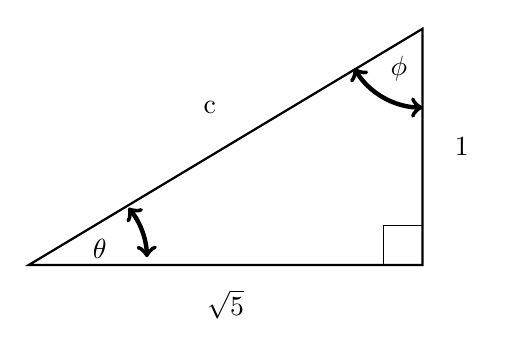
\begin{tikzpicture}
        \draw[black, thick] (0,0) -- (5,0) -- (5,3) -- cycle;
        \draw[ultra thick, <->] (1.5,.1) arc (1:40:1);
        \draw[ultra thick, <->] (5,2) arc (270:210:1);
        % Below nodes are the labels.
            \node[] at (0.9, 0.2) {$\theta$};
            \node[] at (4.7, 2.5) {$\phi$};
            \node[] at (2.5, -0.5) {$\sqrt{5}$};
            \node[] at (5.5, 1.5) {1};
            \node[] at (2.3, 2) {c};
        % This draws the right angle.
            \draw(4.5,0)|-(5,.5);
    \end{tikzpicture}

    \[ (\sqrt{5})^2 + 1^2 = c^2\]
    \[ 6 = c^2\]
    \[ c = \sqrt{6} \]

    Therefore we can state: 

    \[ sin(\theta) = \frac{1}{\sqrt{6}}\]
    \[\boxed{ sin(\theta) = \frac{\sqrt{6}}{6} }\]
\end{solution}


\pagebreak


\begin{problem}[155]
    $sin \left( arcsin \left( \frac{5}{13} \right) + \frac{\pi}{4} \right)$    
\end{problem}

\begin{solution}
    First let's think about this problem in the format of the sum and difference identity. \medskip
    
    We'll let $\alpha = arcsin \left( \frac{5}{13} \right)$ and $\beta = \frac{\pi}{4}$
    
    \medskip
    Before we do anything crazy we need to draw a triangle. Always. No thinking allowed, only triangles. Now you may be thinking "we dont have any sides or angles, we can't do that". Remember, no thinking. Only triangles. Really though, we actually have all of the information we need. Arcsine represents an angle and the x value inside of it also represents a ratio we can use for sides. So, let's get to it. $sin(\alpha) = \frac{opposite}{hypotenuse}$. 
    
        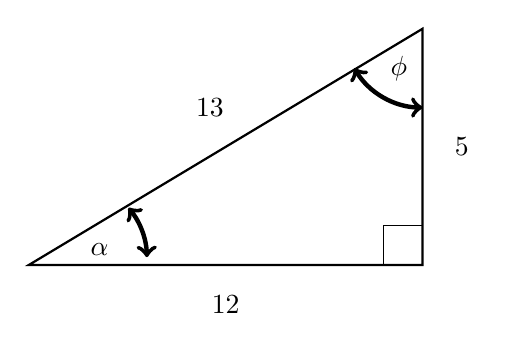
\begin{tikzpicture}
        \draw[black, thick] (0,0) -- (5,0) -- (5,3) -- cycle;
        \draw[ultra thick, <->] (1.5,.1) arc (1:40:1);
        \draw[ultra thick, <->] (5,2) arc (270:210:1);
        % Below nodes are the labels.
            \node[] at (0.9, 0.2) {$\alpha$};
            \node[] at (4.7, 2.5) {$\phi$};
            \node[] at (2.5, -0.5) {12};
            \node[] at (5.5, 1.5) {5};
            \node[] at (2.3, 2) {13};
        % This draws the right angle.
            \draw(4.5,0)|-(5,.5);
    \end{tikzpicture}
    
    Pretend you saw me solve for the last side using the Pythagorean theorem. I'll spare you the calculation. Sweet, now we have all of the information we need. Time to really dig into the sum and difference identity.
    
    \[ sin(\alpha + \beta) = sin\alpha \cdot cos\beta + cos\alpha \cdot sin\beta \]
    
    One last thing, let's solve for all of these so we can substitute them in.
    
    \begin{align}
        sin \left( arcsin \left( \frac{5}{13} \right) \right) = \frac{5}{13} && cos \left( arcsin \left( \frac{5}{13} \right) \right) = \frac{12}{13} \\
        sin\left( \frac{\pi}{4} \right) = \frac{\sqrt{2}}{2} && cos \left( \frac{\pi}{4} \right) = \frac{\sqrt{2}}{2}
    \end{align}
    
    \begin{align}
        sin(\alpha + \beta) &= sin\alpha \cdot 
        cos\beta + cos\alpha \cdot sin\beta \\
        &= \left( \frac{5}{13} \cdot \frac{\sqrt{2}}{2} \right) + \left( \frac{12}{13} \cdot \frac{\sqrt{2}}{2} \right) \\
        &= \left( \frac{5\sqrt{2}}{26} \right) + \left( \frac{12\sqrt{2}}{26} \right)
    \end{align}
    
    \[\boxed{ sin \left( arcsin \left( \frac{5}{13} \right) + \frac{\pi}{4} \right) = \frac{17\sqrt{2}}{26}  }\]
\end{solution}


\pagebreak


\begin{problem}[156]
    $cos(arcsec(3) + arctan(2))$
\end{problem}

\begin{solution}
    Same as the last problem, but this time we need two triangles, not one. Arcsecant will grant us our first triangle and arctangent our second. Let's start with the first. Arcsec(3) represents a ratio of $\frac{3}{1}$ and $arctan(2)$ a ratio of $\frac{2}{1}$. \medskip
    
    Let $arcsec(3) = \alpha$ and $arctan(2) = \beta$
    \medskip
    
    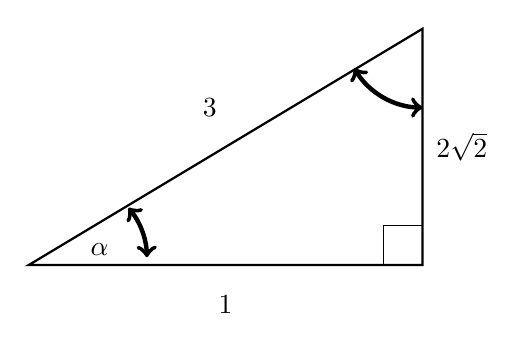
\begin{tikzpicture}
        \draw[black, thick] (0,0) -- (5,0) -- (5,3) -- cycle;
        \draw[ultra thick, <->] (1.5,.1) arc (1:40:1);
        \draw[ultra thick, <->] (5,2) arc (270:210:1);
        % Below nodes are the labels.
            \node[] at (0.9, 0.2) {$\alpha$};
            %\node[] at (4.7, 2.5) {$\phi$};
            \node[] at (2.5, -0.5) {1};
            \node[] at (5.5, 1.5) {$2\sqrt{2}$};
            \node[] at (2.3, 2) {3};
        % This draws the right angle.
            \draw(4.5,0)|-(5,.5);
    \end{tikzpicture}
        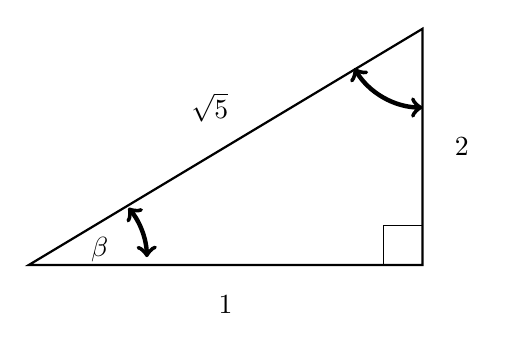
\begin{tikzpicture}
        \draw[black, thick] (0,0) -- (5,0) -- (5,3) -- cycle;
        \draw[ultra thick, <->] (1.5,.1) arc (1:40:1);
        \draw[ultra thick, <->] (5,2) arc (270:210:1);
        % Below nodes are the labels.
            \node[] at (0.9, 0.2) {$\beta$};
            %\node[] at (4.7, 2.5) {$\gamma$};
            \node[] at (2.5, -0.5) {1};
            \node[] at (5.5, 1.5) {$2$};
            \node[] at (2.3, 2) {$\sqrt{5}$};
        % This draws the right angle.
            \draw(4.5,0)|-(5,.5);
    \end{tikzpicture}

    \begin{align}
        cos \left( \alpha \right) = \frac{1}{3} && sin \left( \alpha \right) = \frac{2\sqrt{2}}{3} \\
        cos\left( \beta \right) = \frac{2}{\sqrt{5}} && sin \left( \beta \right) = \frac{2}{\sqrt{5}}
    \end{align}
    
    \begin{align}
        cos(\alpha + \beta) &= cos\alpha \cdot cos\beta - sin\alpha \cdot sin\beta \\
        &= \left( \frac{1}{3} \cdot \frac{1}{\sqrt{5}} \right) - \left( \frac{2\sqrt{2}}{3} \cdot \frac{2}{\sqrt{5}}\right)\\
        &= \frac{\sqrt{5}}{15} - \frac{4\sqrt{10}}{15}
    \end{align}
    
    \[\boxed{ cos(arcsec(3) + arctan(2)) = \frac{ \sqrt{5} - 4\sqrt{10} }{ 15 }  }\]
\end{solution}


\pagebreak

\begin{problem}[165]
    For this exercise, rewrite the quantity as algebraic expressions of x and state the domain on which the equivalence is valid.    

    $sin(arccos(x))$
\end{problem}

\begin{solution}
    Arccosine represents our angle with a ratio of $\frac{x}{1}$ so let's make a triangle. As always.
    
    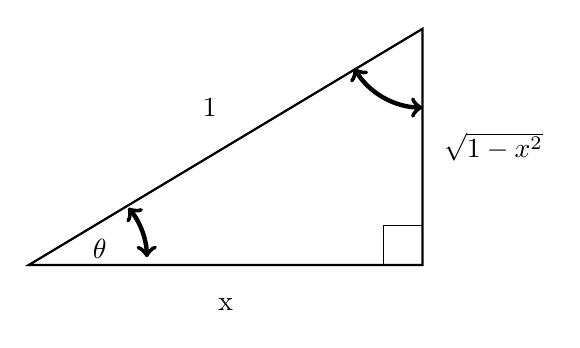
\begin{tikzpicture}
        \draw[black, thick] (0,0) -- (5,0) -- (5,3) -- cycle;
        \draw[ultra thick, <->] (1.5,.1) arc (1:40:1);
        \draw[ultra thick, <->] (5,2) arc (270:210:1);
        % Below nodes are the labels.
            \node[] at (0.9, 0.2) {$\theta$};
            %\node[] at (4.7, 2.5) {$\gamma$};
            \node[] at (2.5, -0.5) {x};
            \node[] at (5.9, 1.5) {$\sqrt{1 - x^2}$};
            \node[] at (2.3, 2) {$1$};
        % This draws the right angle.
            \draw(4.5,0)|-(5,.5);
    \end{tikzpicture}
    
    To show how I solved for the right hand side it's just the standard Pythagorean theorem.
    
    \[ x^2 + b^2 = 1\]
    \[ b^2 = 1 - x^2\]
    \[ b = \sqrt{1 - x^2}\]
    
    Now, we can state what $sin(\theta)$ is equal to.
    
    \begin{align}
        sin(\theta) = \frac{\sqrt{1 - x^2}}{1} \\[+3mm]
        sin(\theta) = \sqrt{1 - x^2}
    \end{align}
    
    Now we just rewrite our function. Our domain is restricted to $-1 \leq x \leq 1$ because we can't have a negative in the square root.
    
    \[\boxed{ sin(arccos(x)) = \sqrt{1 - x^2} \quad for \; -1 \leq x \leq 1 }\]
\end{solution}


\pagebreak


\begin{problem}[185]
    If $sin(\theta) = \frac{x}{2} \; for \; -\frac{\pi}{2} \leq \theta \leq \frac{\pi}{2}$, find an expression for $\theta + sin(2\theta)$ in terms of $x$.
\end{problem}

\begin{solution}
    Triangles. Always triangles.
    
    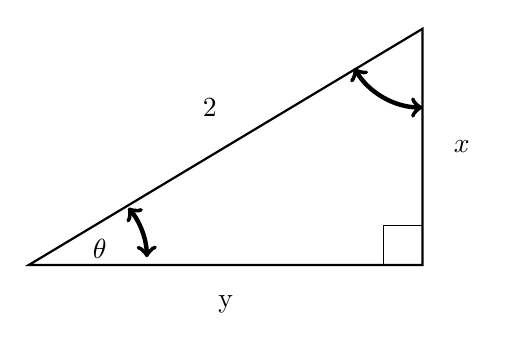
\begin{tikzpicture}
        \draw[black, thick] (0,0) -- (5,0) -- (5,3) -- cycle;
        \draw[ultra thick, <->] (1.5,.1) arc (1:40:1);
        \draw[ultra thick, <->] (5,2) arc (270:210:1);
        % Below nodes are the labels.
            \node[] at (0.9, 0.2) {$\theta$};
            %\node[] at (4.7, 2.5) {$\gamma$};
            \node[] at (2.5, -0.5) {y};
            \node[] at (5.5, 1.5) {$x$};
            \node[] at (2.3, 2) {$2$};
        % This draws the right angle.
            \draw(4.5,0)|-(5,.5);
    \end{tikzpicture}
    
    Solve for y.
    
    \[ y^2 + x^2 = 2^2 \]
    \[ y^2 = 4 - x^2 \]
    \[ y = \sqrt{4 - x^2} \]
    
    Now we plug everything into the given formula. Keep in mind we know that $\theta = arcsin(\frac{x}{2})$. 
    
    \begin{align}
        \theta + sin(2\theta) &= \theta + 2sin(\theta) \cdot cos(\theta) \\
        &= arcsin \left( \frac{x}{2} \right) + \left( 2 \cdot \frac{x}{2} \right) \cdot \left( \frac{\sqrt{4-x^2}}{2} \right) \\
        &= arcsin \left( \frac{x}{2} \right) + \frac{2x \sqrt{4 - x^2}}{4}
    \end{align}
    
    \[\boxed{ if \; sin(\theta) = \frac{x}{2} \; for \; -\frac{\pi}{2} \leq \theta \leq \frac{\pi}{2}, \; then \; \theta + sin(2\theta) =  arcsin \left( \frac{x}{2} \right) + \frac{x \sqrt{4 - x^2}}{2}  }\]
\end{solution}


\pagebreak


\begin{problem}[211]
    A guy wire 1000 feet long is attached to the top of a tower. When pulled taut it touches level ground 360 feet from the base of the tower. What angle does the wire make with the ground? Express your answer using degree measure rounded to one decimal place.
\end{problem}

\begin{solution}
    Don't over-complicate this one. Lets start with a triangle, as always!    
    
    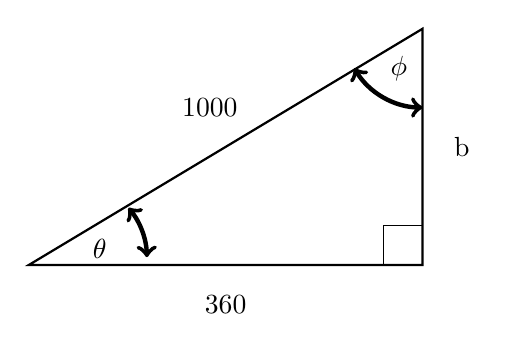
\begin{tikzpicture}
        \draw[black, thick] (0,0) -- (5,0) -- (5,3) -- cycle;
        \draw[ultra thick, <->] (1.5,.1) arc (1:40:1);
        \draw[ultra thick, <->] (5,2) arc (270:210:1);
        % Below nodes are the labels.
            \node[] at (0.9, 0.2) {$\theta$};
            \node[] at (4.7, 2.5) {$\phi$};
            \node[] at (2.5, -0.5) {$360$};
            \node[] at (5.5, 1.5) {b};
            \node[] at (2.3, 2) {1000};
        % This draws the right angle.
            \draw(4.5,0)|-(5,.5);
    \end{tikzpicture}
    
    So to solve for $\theta$ we can plug $arccos \left( \frac{360}{1000} \right)$ into our calculator (or programming language) of choice. 
    
    \[ arccos \left( \frac{360}{1000} \right) = 1.2 (radians)\]
    
    Now we just convert! 
    
    \[1.2 \cdot \frac{180}{\pi} = 68.75\]
    \[ \theta = 69\degree\]
\end{solution}


\begin{problem}[212]
    At Cliffs of Insanity Point, The Great Sasquatch Canyon is 7117 feet deep. From that point, a fire is seen at a location known to be 10 miles away from the base of the sheer canyon wall. What angle of depression is made by the line of sight from the canyon edge to the fire? Express your answer using degree measure rounded to one decimal place.
\end{problem}

\begin{solution}
    First thing first, let's convert our units and make a diagram. 
    
    \[ 7117ft \cdot \frac{1mile}{5280ft} = 1.347 miles\]
    
        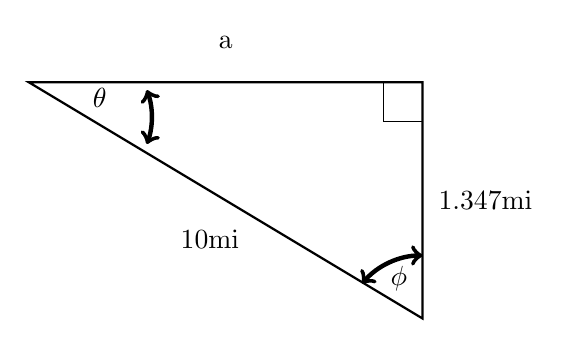
\begin{tikzpicture}
        \draw[black, thick] (0,0) -- (5,0) -- (5,-3) -- cycle;
        \draw[ultra thick, <->] (1.5,-.1) arc (20:-20:1);
        \draw[ultra thick, <->] (5,-2.2) arc (90:140:1);
    % Below nodes are the labels.
        \node[] at (0.9, -0.2) {$\theta$};
        \node[] at (4.7, -2.5) {$\phi$};
        \node[] at (2.5, 0.5) {a};
        \node[] at (5.8, -1.5) {1.347mi};
        \node[] at (2.3, -2) {10mi};
    % This draws the right angle.
        \draw(4.5,0)|-(5,-.5);
    \end{tikzpicture}
    
    
    \[ arcsin \left( \frac{1.347}{10} \right) = 0.135 (radians)\]
    \[ 0.135 \cdot \frac{180}{\pi} = 7.73\degree\]
    \[\boxed{ \theta = 8\degree }\]
\end{solution}


\pagebreak


\begin{problem}[213]
Shelving is being built at the Utility Muffin Research Library which is to be 14 inches deep. An 18-inch rod will be attached to the wall and the underside of the shelf at its edge away from the wall, forming a right triangle under the shelf to support it. What angle, to the nearest degree, will the rod make with the wall?
\end{problem}

\begin{solution}
    This is the same as the previous problem. This time we can just use arctangent instead of arcsine. 
    
    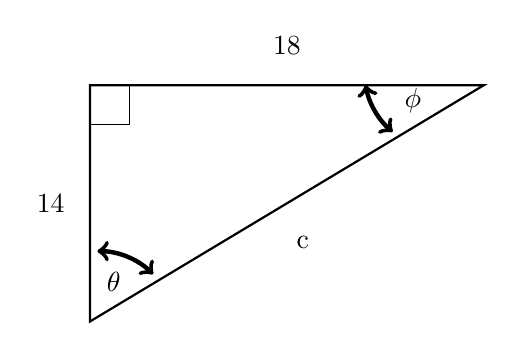
\begin{tikzpicture}
    \draw[black, thick] (0,0) -- (-5,0) -- (-5,-3) -- cycle;
    \draw[ultra thick, <->] (-1.5,0) arc (190:230:1);
    \draw[ultra thick, <->] (-4.2,-2.4) arc (45:90:1);
    % Below nodes are the labels.
        \node[] at (-0.9, -0.2) {$\phi$};
        \node[] at (-4.7, -2.5) {$\theta$};
        \node[] at (-2.5, 0.5) {18};
        \node[] at (-5.5, -1.5) {14};
        \node[] at (-2.3, -2) {c};
    % This draws the right angle.
        \draw(-4.5,0)|-(-5,-.5);
\end{tikzpicture}

    \[ arctan \left( \frac{18}{14} \right) = 0.909 (radians)\]
    \[ 0.909 \cdot \frac{180}{\pi} = 52\degree\]
    \[\boxed{\theta = 52\degree}\]
\end{solution}


\begin{problem}[214]
    A parasailor is being pulled by a boat on Lake Ippizuti. The cable is 300 feet long and the parasailor is 100 feet above the surface of the water. What is the angle of elevation from the boat to the parasailor? Express your answer using degree measure rounded to one decimal place.
\end{problem}

\begin{solution}
    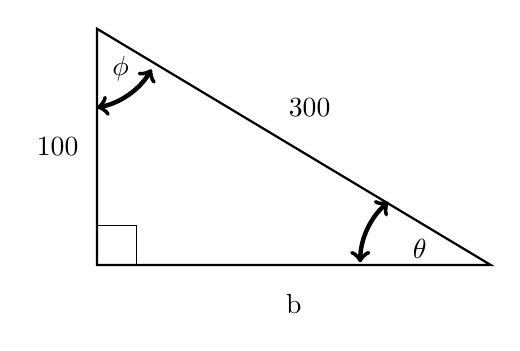
\begin{tikzpicture}
    \draw[black, thick] (0,0) -- (-5,0) -- (-5,3) -- cycle;
    \draw[ultra thick, <->] (-1.3,.8) arc (130:180:1);
    \draw[ultra thick, <->] (-5,2) arc (280:330:1);
    % Below nodes are the labels.
        \node[] at (-0.9, 0.2) {$\theta$};
        \node[] at (-4.7, 2.5) {$\phi$};
        \node[] at (-2.5, -0.5) {b};
        \node[] at (-5.5, 1.5) {100};
        \node[] at (-2.3, 2) {300};
    % This draws the right angle.
        \draw(-4.5,0)|-(-5,.5);
\end{tikzpicture}

You know how it goes, we can use arcsine to solve this easily.

\[ arcsine \left( \frac{100}{300} \right) = 0.339 \]
\[ 0.339 \cdot \frac{180}{\pi} = 19.5\degree\]
\[ \theta = 19.5\degree \]
\end{solution}


\pagebreak

References

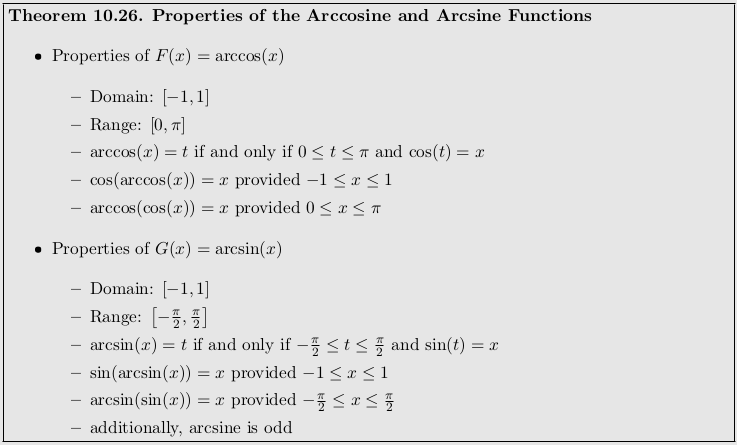
\includegraphics[width=6inches, scale=1.0]{images/arccos_and_arcsin.png}

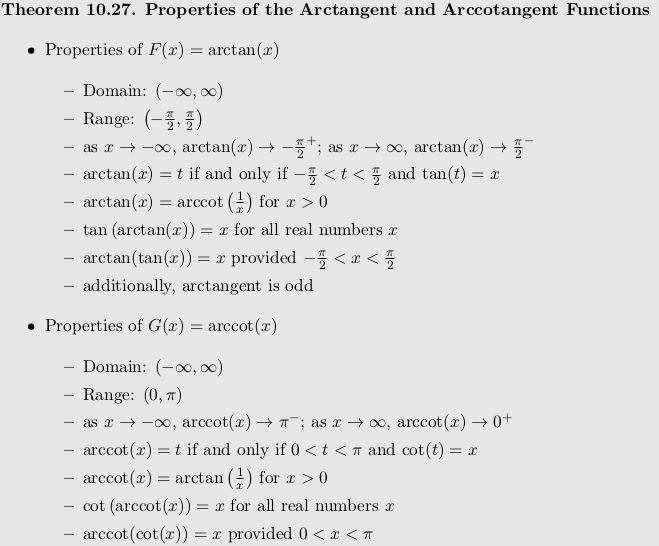
\includegraphics[width=6inches, scale=1.0]{images/arctan_and_arccotan.png}

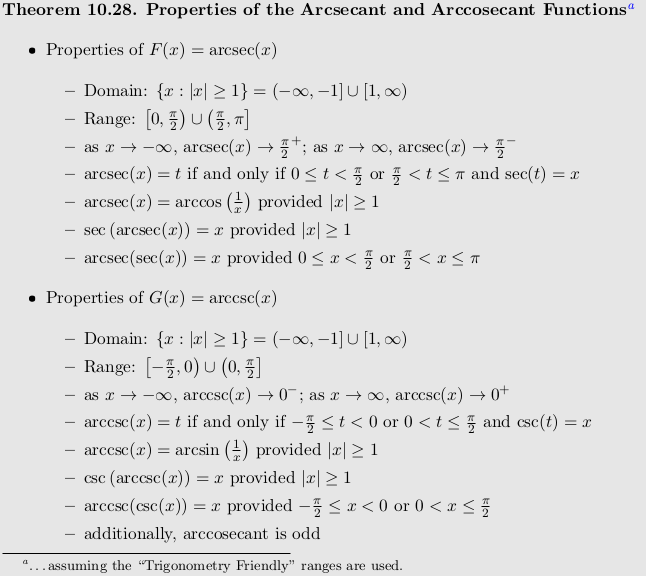
\includegraphics[width=6inches, scale=1.0]{images/arcsec_and_arccsc.png}
\end{document}